\documentclass[10pt, a4paper]{scrartcl}

\usepackage{vorschule}
\usepackage[
    typ=ab,
    fach=Informatik,
    lerngruppe={EF},
    nummer={I.4},
    module={Symbole,Lizenzen},
    seitenzahlen=keine,
    farbig,
    lizenz=cc-by-nc-sa-4,
]{schule}

\usepackage[
	kuerzel=Ngb,
	reihe={Informationen, Daten und Codierung},
	version={2020-09-7},
]{ngbschule}

\author{J. Neugebauer}
\title{Fehlerkorrigierende Codes II}
\date{\Heute}

\setzeAufgabentemplate{ngbnormal}

\usepackage{qrcode}

\begin{document}

\ReiheTitel

\begin{multicols}{2}
Die folgende Tabelle zeigt noch einmal die Codierung der vier möglichen Nachrichten aus zwei Bits:
\begin{center}
\begin{tabular}{cc}
	Nachricht & Codewort \\\hline
	\code{00} & \code{000000} \\
	\code{01} & \code{010111} \\
	\code{10} & \code{101011} \\
	\code{11} & \code{111100} \\
\end{tabular}
\end{center}

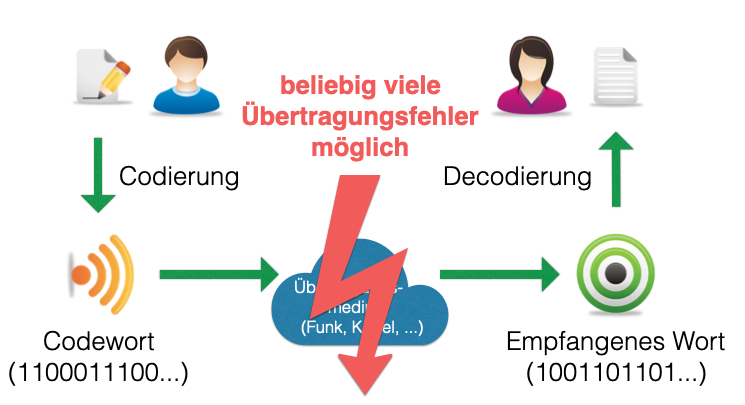
\includegraphics[height=4.5cm]{EF-AB.I.4-Abb_1}
\end{multicols}

\begin{infobox}
	Schaut man sich zwei Codewörter an (z.B. \code{010111} und \code{101011}), so stimmen sie in einigen Bits überein und in anderen unerscheiden sie sich. Im Beispiel oben sind die hinteren zwei Bits gleich, der Rest ich verschieden. Die \textbf{Anzahl} der Bits, in denen sich zwei Codewörter \emph{A} und \emph{B} unterscheiden, nennt man \enquote{\emph{Hamming-Distanz zwischen A und B}}. Die beiden Codewörter im Beispiel sind in 4 Bits verschieden, also ist ihrer Hamming-Distanz gleich 4 (man schreibt $d(010111, 101011) = 4$).
	
	Es könnte nun durch genau 4 Übertragungsfehler passieren, dass aus dem Codewort \code{010111} das Codewort \code{101011} wird, ohen das dies auffällt (das empfangene Wort ist ja wieder ein gültiges Wort). Treten \emph{weniger} als 4 Fehler auf, so entstehen Worte, die nicht gültig sind. Der Empfänger erkennt also, dass die Übertragung fehlerhaft war (Abb. 2 zeigt die beiden gültigen Codeworte (schwarz) und drei ungültige (weiß) dazwischen).
	
	\begin{wrapfig}
	\begin{wrapfigure}{r}{7cm}
	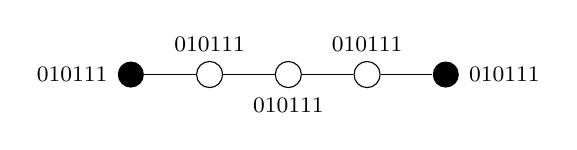
\begin{tikzpicture}[word/.style={circle,fill=black},err/.style={circle,fill=white,draw=black}]
		\node[word,label=left:{\code{\footnotesize 010111}}] (a) {};
		\node[err,right of=a,label=above:{\code{\footnotesize 010111}}] (b) {};
		\node[err,right of=b,label=below:{\code{\footnotesize 010111}}] (c) {};
		\node[err,right of=c,label=above:{\code{\footnotesize 010111}}] (d) {};
		\node[word,right of=d,label=right:{\code{\footnotesize 010111}}] (e) {};
		\draw (a) -- (b) -- (c) -- (d) -- (e);
	\end{tikzpicture}
	\emph{Abb. 2: Ungültige Worte zwischen \code{010111} und \code{101011}}
	\end{wrapfigure}
	Tritt nur \emph{ein} Übertragungsfehler auf (z.B. wird \code{010111} zu \code{110111}), so wird der Fehler erkannt und kann sogar korrigiert werden. Bei \emph{zwei} Fehlern (z.B. wird \code{010111} zu \code{100111}) ist der Fehler nicht korrigierbar! \emph{Ist dir klar, warum?}
	\end{wrapfig}
\end{infobox}

\begin{aufgabe}
	Berechne auch für die übrigen Kombinationen von Codewörtern aus der Tabelle oben die Hamming-Distanz. Was fällt dir auf?
	
	Was bedeutet es praktisch, wenn zwei Codewörter die Hamming-Distanz 1 haben?
\end{aufgabe}

\begin{aufgabe}
	Als Empänger erhältst du das Wort \code{111011}. Dieses Wort ist offensichtlich falsch übertragen worden. Als welches Codewort würdest du es interpretieren und wie lautet somit die gesendete Nachricht?
\end{aufgabe}

\begin{aufgabe}
	Als Empänger erhältst du das Wort \code{111111}. Dieses Wort gehört nicht zu den gültigen Codewörtern, es ist also ein Übertragungsfehler aufgetreten. Begründe, warum das Wort nicht sicher korrigiert werden kann.
\end{aufgabe}

\begin{aufgabe*}
	Es ist nicht besonders effizient, für \textbf{zwei} Nachrichtenbits \textbf{vier} Prüfbits zu versenden. Kannst du einen Code für die vier 2-Bit Nachrichten von oben  entwerfen, der mit \emph{weniger} als vier Prüfbits auskommt, aber trotzdem einen Fehler korrigieren kann? Wie viele Übertragungsfehler kann dein Code erkennen?
\end{aufgabe*}

\end{document}
